%%%---------------------------------------------------------
%% Anhang, falls erforderlich
%%---------------------------------------------------------
\appendix                %% appendix ist keine Umgebung!

\pagenumbering{roman}
\section{Anhang}%

\begin{figure}[h!]
	\centering
	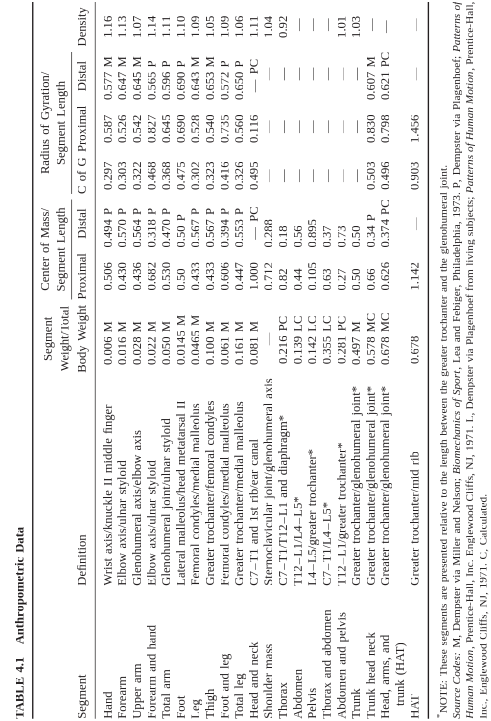
\includegraphics[width=.9\linewidth]{bilder/anhang/anthrop_Tabelle}
	\caption[Anthropometrische Tabelle]{Anthropometrische Tabelle aus \textcite{winter2009biomechanics}}
	\label{fig:antrop_Tabelle}
\end{figure}

\section*{Inverse Kinetik}
\subsection*{Berechnung Fußsegment}
\begin{minipage}{.5\linewidth}
\paragraph{Kräfte in X-Richtung}
\begin{equation*}
\begin{split}
\sum F_x &= m \cdot a_x\\
F_x + F_{ax} &= m_{foot} \cdot a_{x foot}\\
F_x &= m_{foot} \cdot a_{x foot} - F_{ax} 
\end{split}
\end{equation*}

\paragraph{Kräfte in Y-Richtung}
\begin{equation*}
\begin{split}
\sum F_y &= m \cdot a_y\\
F_y + F_{ay} + F_g &= m_{foot} \cdot a_{y foot}\\
F_y &= m_{foot} \cdot a_{y foot} -  F_{ay} - F_g
\end{split}
\end{equation*}
\end{minipage}%
\begin{minipage}{.5\linewidth}
	\centering
	\includegraphics[width=\linewidth]{bilder/anhang/foot_segment}
	\captionof{figure}{Berechnung des Fußsegmentes. Abbildung aus Skript zur Datenauswertung (Owsianowsky 2016)}
	\label{fig:foot_segment}
\end{minipage}

\paragraph{Momente um Z-Achse}
\begin{equation*}
\begin{split}
\sum M &= I_o \cdot \alpha\\
M_a + F_{ay} \cdot (x_a - x_g) + F_{ax} \cdot (y_g-y_a) + F_x \cdot (y_a - y) + F_y \cdot (x -x_g) &= I_o \cdot \alpha\\
M_a = I_o \cdot \alpha - F_{ay} \cdot (x_a - x_g) - F_{ax} \cdot (y_g-y_a) - F_x \cdot (y_a - y) - F_y \cdot (x -x_g)
\end{split}
\end{equation*}

\subsection*{Berechnung Beinsegment}
\begin{minipage}{.5\linewidth}
	\paragraph{Kräfte in X-Richtung}
	\begin{equation*}
	\begin{split}
	\sum F_x &= m \cdot a_x\\
	F_{px} + F_{dx} &= m_{foot} \cdot a_{x foot}\\
	F_{dx}&= m_{foot} \cdot a_{x foot} - F_{px} 
	\end{split}
	\end{equation*}
	
	\paragraph{Kräfte in Y-Richtung}
	\begin{equation*}
	\begin{split}
	\sum F_y &= m \cdot a_y \\
	F_{py} + F_{dy} + F_g &= m_{foot} \cdot a_{y foot}\\
	F_{py} &= m_{foot} \cdot a_{y foot} -  F_{dy} - F_g
	\end{split}
	\end{equation*}
\end{minipage}%
\begin{minipage}{.5\linewidth}
	\includegraphics[width=\linewidth]{bilder/anhang/leg_segment}
	\captionof{figure}{Berechnung des Beinsegmentes. Abbildung aus Skript zur Datenauswertung (Owsianowsky 2016)}
	\label{fig:leg_segment}
\end{minipage}



\paragraph{Momente um Z-Achse}
\begin{equation*}
	\begin{split}
		\sum M &= I_o \cdot \alpha\\
		M_d + M_p + F_{py} \cdot (x_p - x_g) + F_{px} \cdot (y_g-y_d) + F_{dx} \cdot (y_g - y_d) + F_{dy} \cdot (x_d -x_g) &= I_o \cdot \alpha\\
		M_p = I_o - M_d - F_{py} \cdot (x_p - x_g) - F_{px} \cdot (y_g-y_d) - F_{dx} \cdot (y_g - y_d) - F_{dy} \cdot (x_d -x_g)
	\end{split}
\end{equation*}

\section*{Zusammenfassung der Waagenkanäle}
\begin{table}[h!]
	\centering
	\caption{Waagenkanäle und von den 4 Kraftsonden eingehende Signale}
	\label{tab:Kanäle}
	\begin{tabular}{c c}
		\toprule
		Kanal & Kraftwerte der 4 Kraftsonden \\
		\midrule
		K1	& x1, x2\\
		K2	& x3, x4\\
		K3	& y1, y4\\
		K4 	& y2, y3\\
		K5	& z1\\
		K6	& z2\\
		K7	& z3\\
		K8	& z4\\
		\bottomrule
	\end{tabular}
\end{table}

\begin{table}[h!]
\centering
\caption{Zusammenfassung der Kanäle in Kraftrichtungen}
\label{tab:Kräfte}
\begin{tabular}{c l}
	\toprule
	Kraft & Kanal \\
	\midrule
	$F_x$	& K1 + K2\\
	$F_y$	& K3 + K4\\
	$F_z$	& K5 + K6 + K7 + K8\\
	$M_x$	& b(K5 +K6 + K7 +K8)\\
	$M_y$	& a (-K5 + K6 + K7 -K8)\\
	$M_z$	& b (-K1 + K2) + a(K3 - K4)\\
	\bottomrule
\end{tabular}
\end{table}

\begin{minipage}{.5\textwidth}
	\includegraphics[width=\linewidth]{bilder/anhang/kraftmess}
	\captionof{figure}{Berechnung des Beinsegmentes. Abbildung aus Skript zur Datenauswertung (Owsianowsky 2016)}
	\label{fig:kraftmess}
\end{minipage}